\section{Background Information}
\subsection{Vierobot Company Limited}
\subsubsection {Basic information}
\begin{figure}[H]
	\centering
	
\includegraphics[width = 0.25\textwidth]{images/vierobot_logo.png}
	\caption{Vierobot Logo}
\end{figure}
\begin{itemize}
	\item \textbf{Company Name}: Vierobot Company Limited
	\item \textbf{Slogan}: Quality, Precision, and Reliability
	\item \textbf{Location}: 10/20, Street 30, Linh Dong Ward, Thu Duc City, HCMC
	\item \textbf{Industry}: Machinery Manufacturing
	\item \textbf{Website}: \href{https://viercycle.com/}{viercycle.com}
\end{itemize}

The company provides IoT solutions, have their own eBike brand VierCycle and eBike service KUTKIT.

Because my main job at the company is developing devices of VierCycle, so I want to introduce more about it.

\subsubsection{VierCycle}

At VierCycle, people make high-quality eBike drive systems with high-tech integration and cloud-based software applications, and also provides comprehensive eBike solutions\cite{viercycle}.

VierCycle offers a wide range of applications, from daily commutes, weekend rides to leisure activities while prioritizing safety, reliability and performance.

\begin{figure}[H]
	\centering
	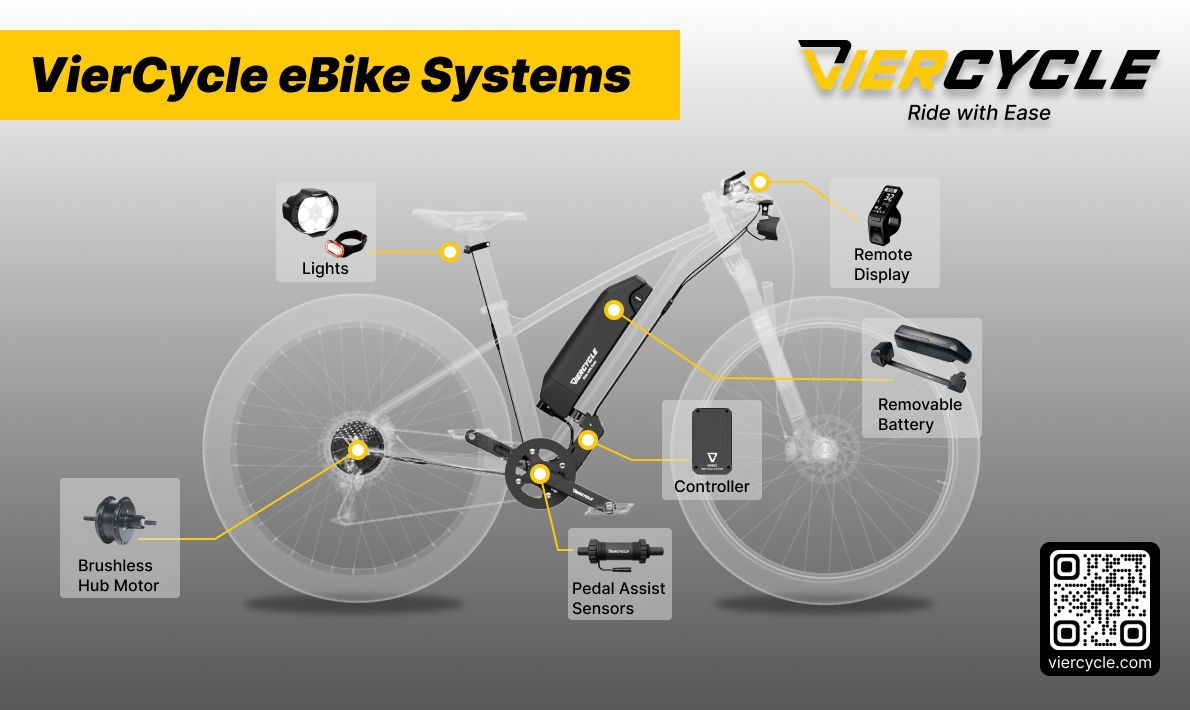
\includegraphics[width = 0.75\textwidth]{images/viercycle_ebike_systems.jpeg}
	\caption{VierCycle eBike Systems. \textit{Source: \href{https://www.linkedin.com/posts/viercycle_viercycle-ridewithease-emobility-activity-7121323454666088448-dchL?utm_source=share&utm_medium=member_desktop}{LinkedIn}}}
	\label{fig: viercycle_ebike_systems}
\end{figure}

\subsection{My position and responsibilities}

At Vierobot, I am working as an Embedded System Intern.

I take part in developing the firmware of company's products. More specific, I have worked with communication protocols between parts of device system. As you can see at Figure \ref{fig: viercycle_ebike_systems}, I contributed to the communication between Remote Display and Controller.

Beside that, I also lend a hand with other activities of the company like repairing devices, joining exhibition,...

My main responsibilities are:

\begin{itemize}
	\item {Researching, writing documents for new parts}
	\item {Implementing, developing features for devices}
\end{itemize}

